\NoBgThispage
\chapter{Autonomous Driving and HD Maps}
The purpose of this chapter is to provide an overview, before delving into the specifics, to first understand what High Definition (HD) maps are and their significance in the field of autonomous driving.

\section{Introduction to Autonomous Driving (AD)}
The concept of \textit{autonomous driving} has evolved from a theoretical idea to a rapidly advancing field with profound technological, societal, and legal implications. Autonomous vehicles (AVs) hold the potential to revolutionize transportation by improving safety, reducing congestion, and enhancing mobility \cite{9695620}. The technological backbone of this transformation involves advanced sensors, machine learning and deep learning algorithms, vehicle-to-everything (V2X) communication, and real-time decision-making algorithms.

At the core of understanding the complexity and potential of autonomous vehicles lies the classification system developed by the Society of Automotive Engineers (SAE)\footnote{The Society of Automotive Engineers (SAE) is a global organization that established a standardized framework for defining and categorizing levels of driving automation. This framework is intended to clarify the roles of human drivers and automated systems, ensuring consistent standards for safety and functionality across various levels of automation.} \cite{SAE_J3016_202104}, which defines the various stages of vehicle automation.

The SAE International established a six-tier classification system in 2014, which was refined in subsequent years, to standardize the levels of driving automation across the industry. The levels range from Level 0, where no automation exists, to Level 5, representing full automation. Each level represents a step toward the ultimate goal of a fully autonomous vehicle, and these levels are essential in understanding the current and future development of AV technology \cite{9881892}.

\begin{figure}
    \centering
    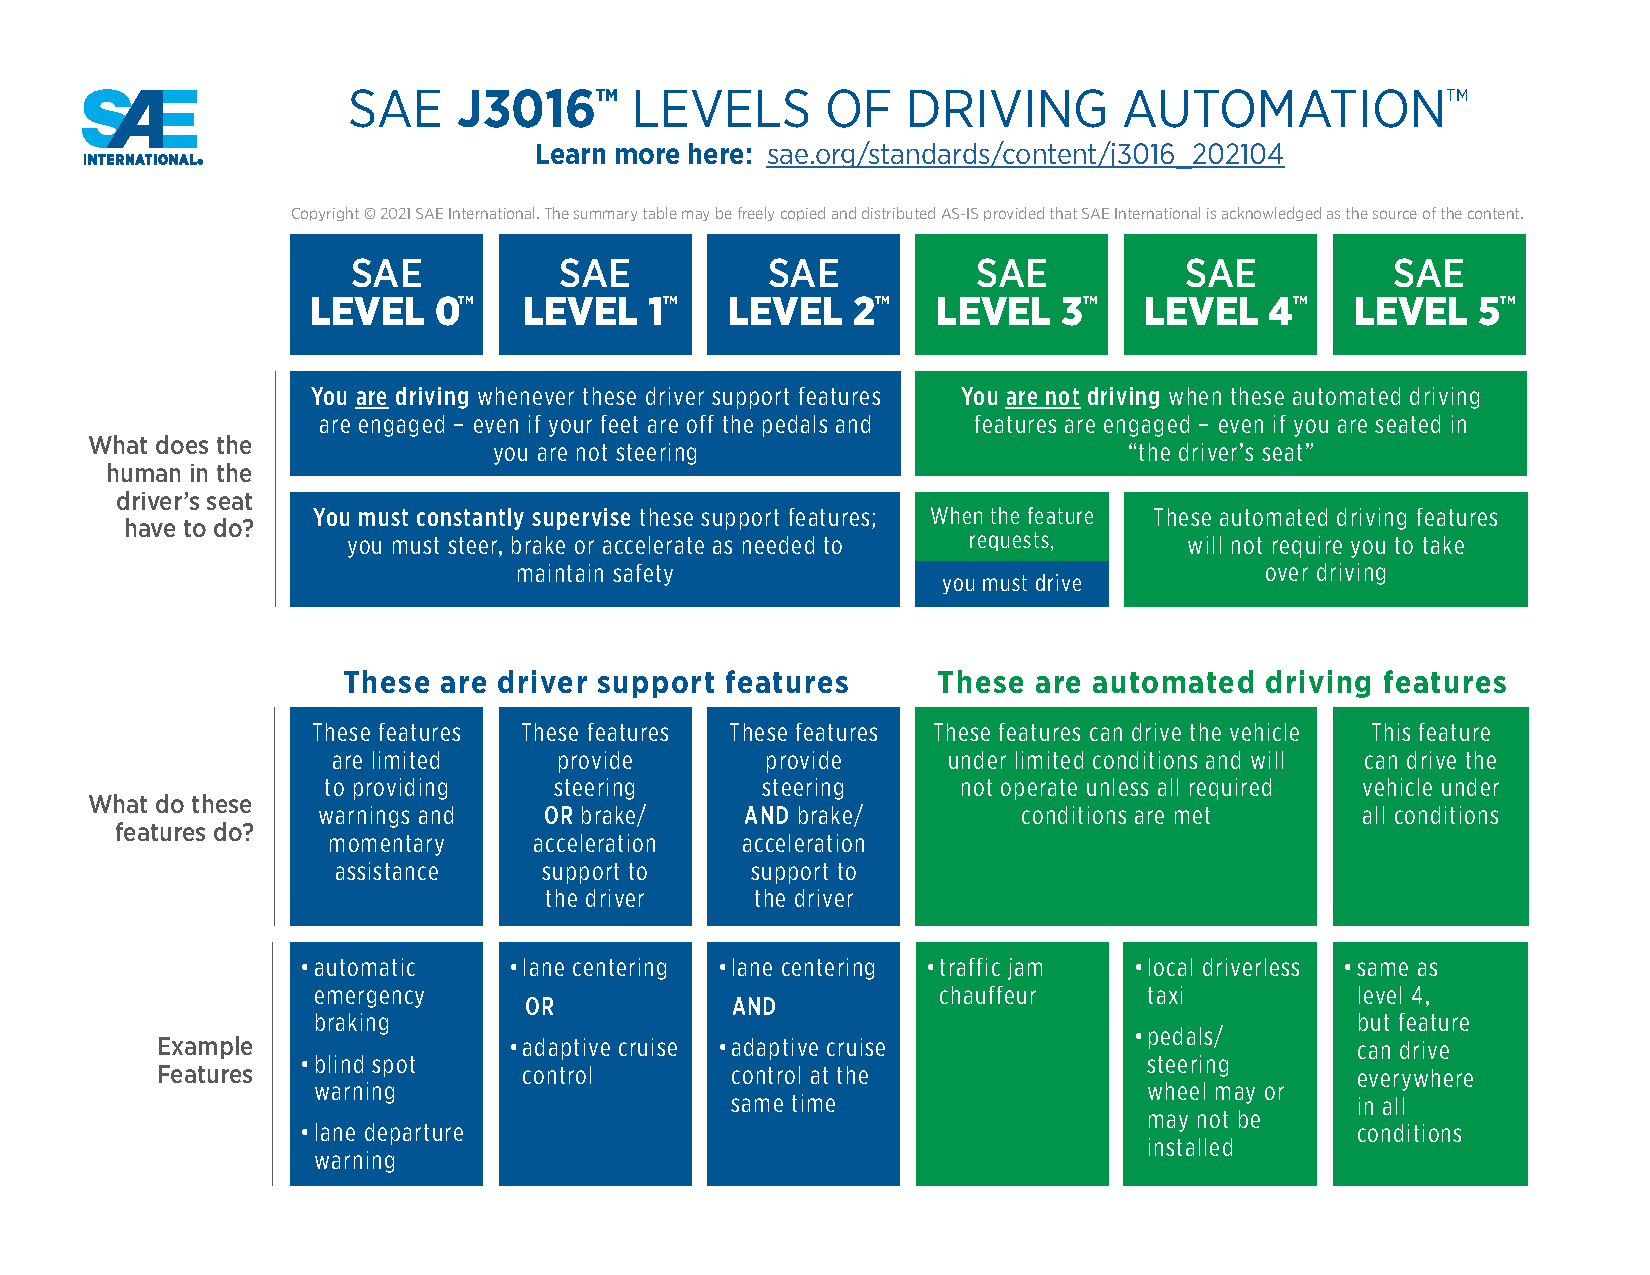
\includegraphics[width=1\linewidth]{LateX//figs/sae-j3016-visual-chart_5.3.21.pdf}
    \caption{SAE J3016 Levels of Driving Automation graphic}
    \label{fig:enter-label}
\end{figure}

\begin{itemize}
    \item Level 0: No Automation – At this level, the human driver is fully responsible for all tasks, though the vehicle may provide warnings or momentary assistance, such as automatic emergency braking (SAE J3016).
    \item Level 1: Driver Assistance – Vehicles at this level are equipped with systems like adaptive cruise control, where the driver remains in control but can benefit from limited automated assistance in specific scenarios.
    \item Level 2: Partial Automation – Level 2 vehicles can control both steering and acceleration/deceleration under certain conditions, but the human driver must remain attentive and ready to take over at any time.
    \item Level 3: Conditional Automation – At this level, the vehicle can manage most driving tasks, but the driver must be available to overtake when requested by the system. This level marks a significant milestone as the vehicle can make decisions autonomously under specific circumstances.
    \item Level 4: High Automation – Vehicles at Level 4 can operate without human intervention in certain conditions or geographic areas. However, a driver may still be required for situations outside the vehicle's operational design domain.
    \item Level 5: Full Automation – At the highest level, the vehicle can operate autonomously in all conditions and environments, without any need for human input. This level predicts a future where transportation no longer relies on human drivers.
\end{itemize}

The progression through these levels is not just a technical challenge but also involves addressing ethical, regulatory, and safety concerns. Autonomous driving technology is a complex field that incorporates artificial intelligence, sensor fusion, human-machine interaction, and cybersecurity. 

Currently, the industry has achieved partial automation (level 3) in some commercial vehicles, allowing the vehicle to handle certain driving tasks with human oversight. The system is designed to activate only on pre-approved roads, meaning it won’t work just anywhere. For example, this functionality is currently available on certain highways across key regions and major city areas within approved states, linking certain metropolitan zones with limited-access highways \cite{bmw2024}.

Looking ahead, certain companies have announced plans to reach level 4 automation in the near future, aiming for vehicles that can perform all driving tasks under specific conditions without human intervention. This progression is closely tied to the rise of the robo-taxi\footnote{A robo-taxi is an autonomous vehicle designed to operate as a taxi service without a human driver. Equipped with high levels of automation (at least level 4), these vehicles can navigate, pick up, and drop off passengers independently within specific operational areas or conditions} phenomenon, where fully autonomous vehicles could provide ride-hailing services without a driver. Achieving these higher levels of automation will demand sophisticated mapping and a precise, real-time reconstruction of the environment around the vehicle.

\section{HD Maps: Definition and Importance}

Maps are essentials to the development and implementation of autonomous driving systems, that help with navigation and understanding the surroundings. Self-driving cars use many types of maps that enable precise navigation and an accurate environmental perception. 

\subsection{SD Maps}
The simplest of these are Standard-Definition (SD) maps, which are typically used in conventional GPS-based navigation systems. SD maps show a complete map of the roads, points of interest (POIs) like landmarks and businesses, basic journey information, and sometimes also traffic data. They are the digital equivalent to traditional paper maps, containing essential details needed to navigate from point A to point B, such as road networks with basic shapes and directions, addresses, and notable locations \cite{Mudduluru_SD_vs_HD_Maps, Chiang2021}.
However SD maps alone are not enough for autonomous driving, where a vehicle must take decisions independently and requires a clear sense of its environment, they lack the fine-grained detail and real-time data necessary for the complex decision-making involved in this field.
\begin{figure}[H]
    \centering
    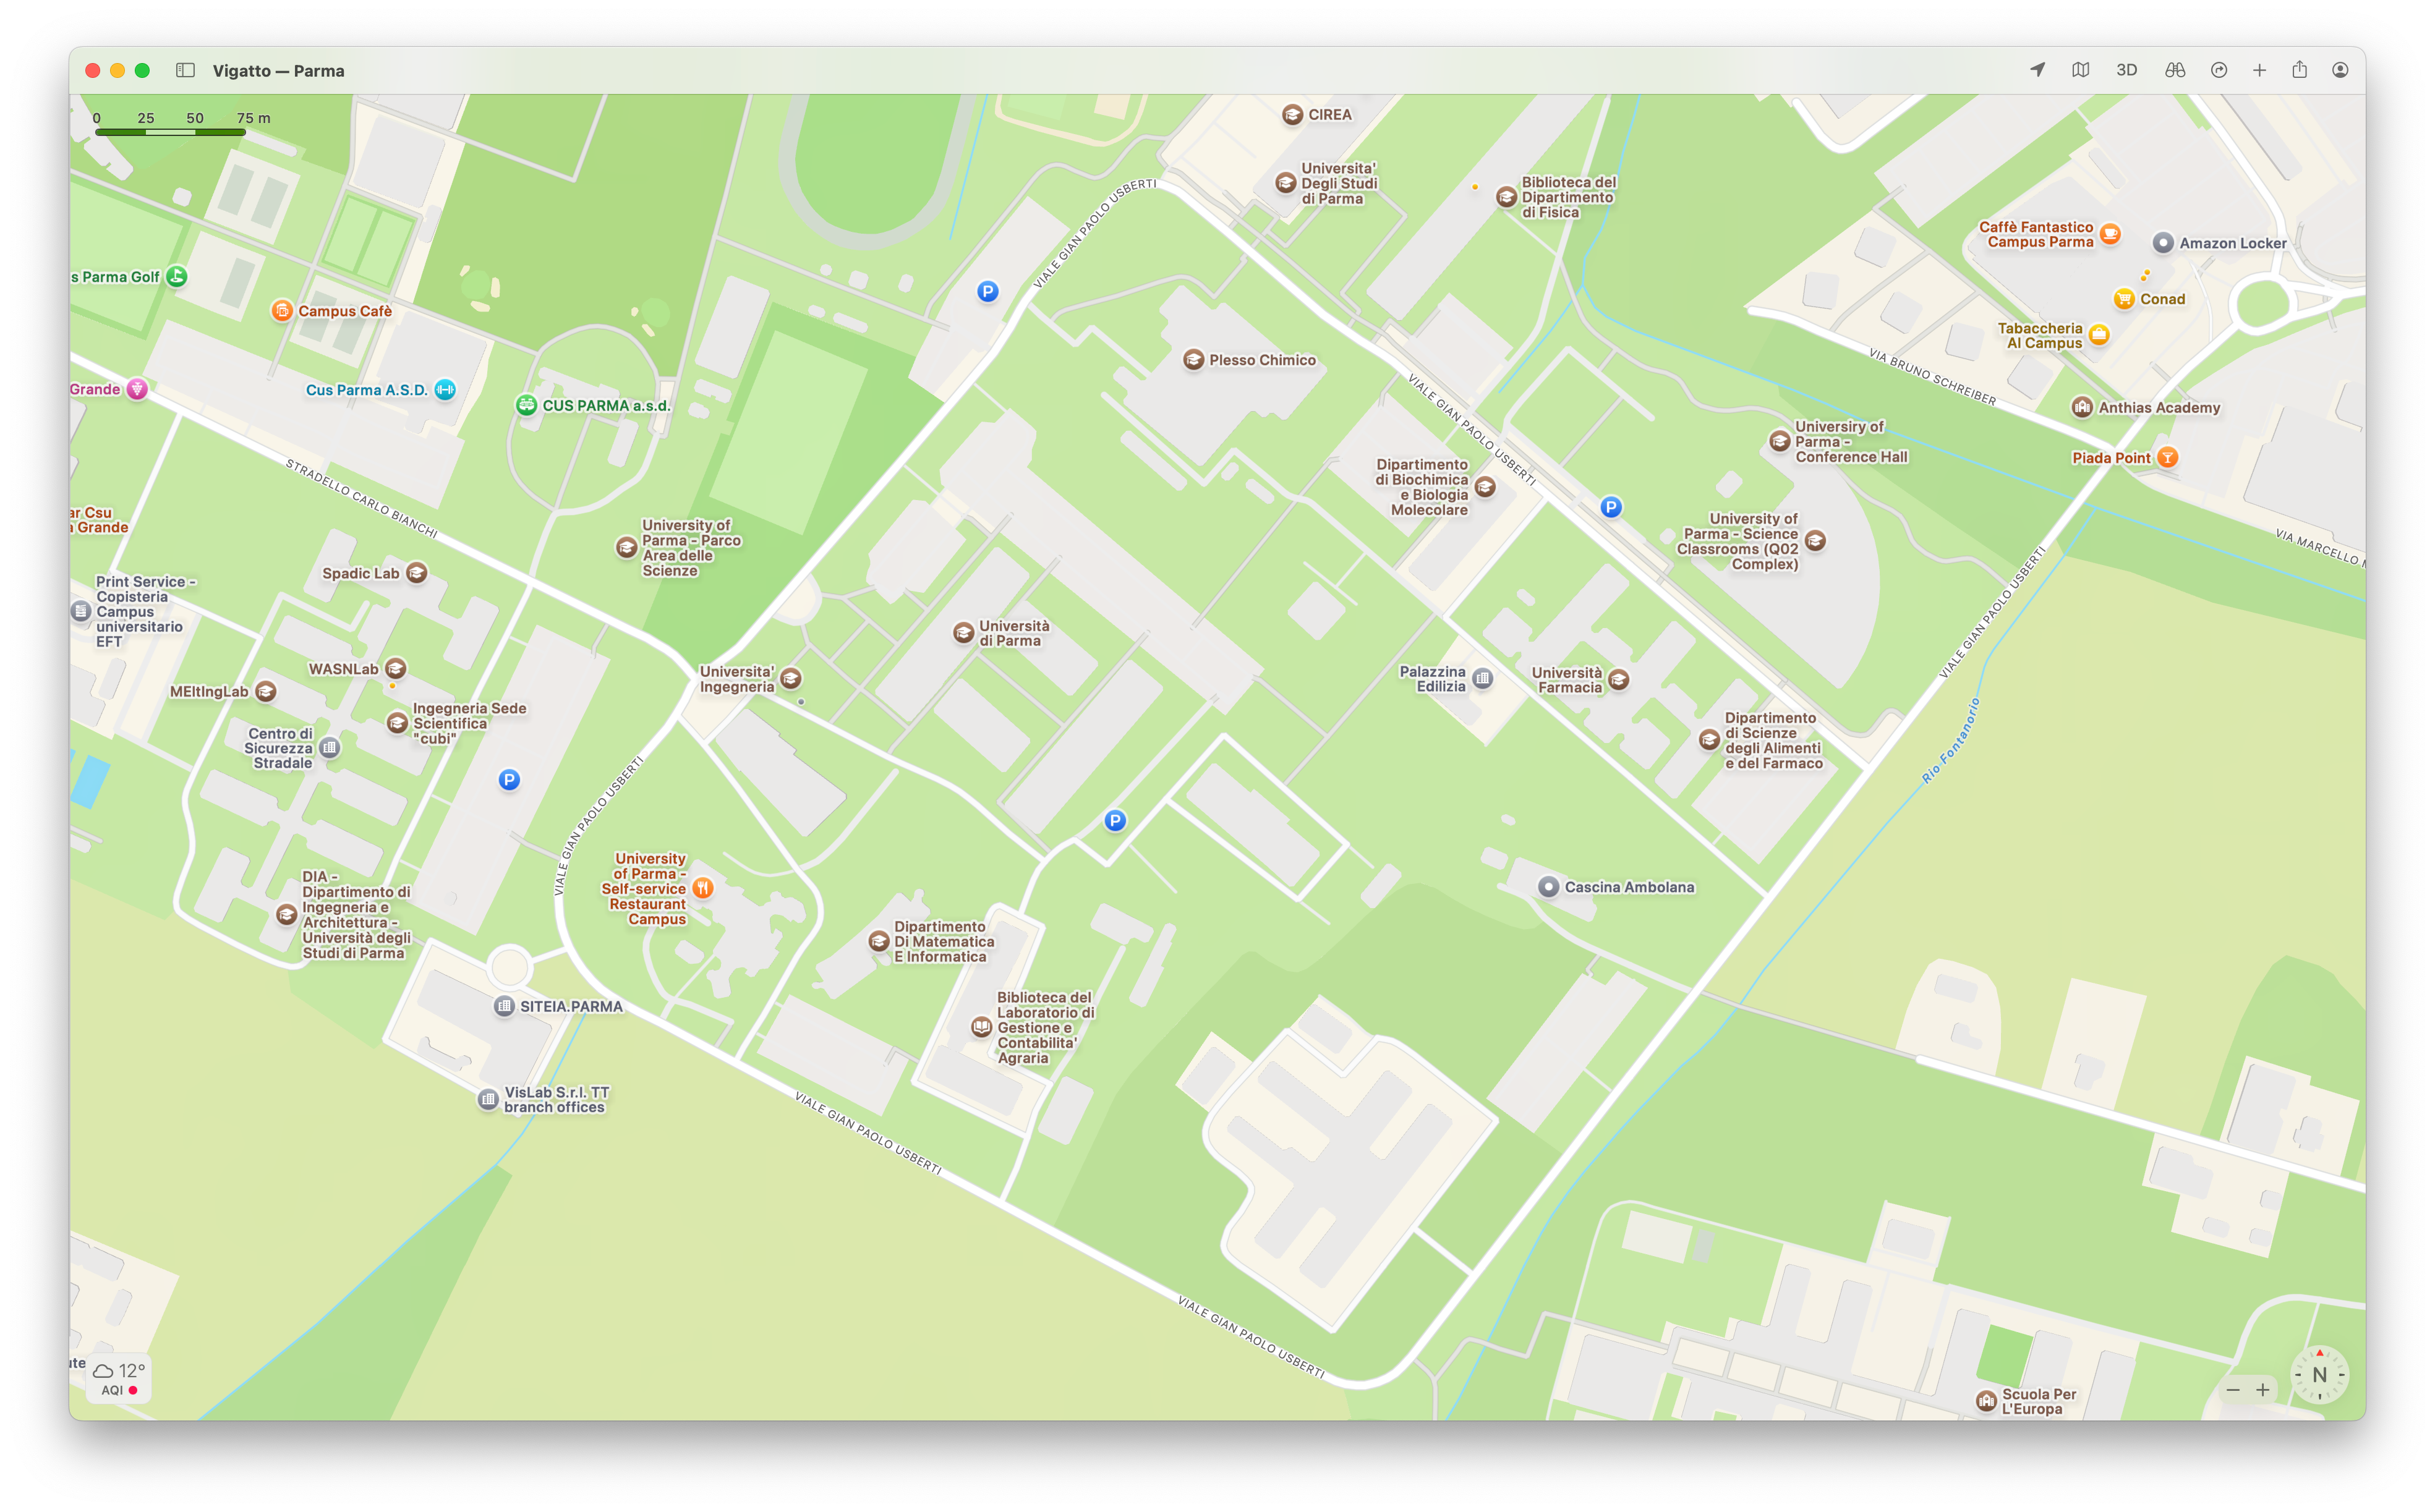
\includegraphics[width=0.65\linewidth]{LateX//figs/SD_MAP.png}
    \caption{Brevissima descrizione e indicare anche la fonte -> AppleMaps, provided by TomTom}
    \label{fig:enter-label}
\end{figure}

\subsection{Topological Maps}
Topological maps, which are representations of the environment focusing on the connectivity of locations rather than geometric details, began to be explored in autonomous driving (AD) around the 2000s. They introduce a layer of connectivity that can be helpful in robot navigation. These maps represent environments through a graph structure, where intersections, pathways, and connections between road segments are shown without needing precise geometric data \cite{li2020survey}. For example, a topological map of a subway system uses nodes to represent stations, with edges representing navigable paths between them. \cite{8105770}
Topological maps provide advantages by saving only relevant information at points called nodes, which represent specific situations, places, or landmarks. They require less memory than metric maps, which memorizes every pixel in the environment. These nodes are connected by edges, defining navigable paths between locations, and can store useful data, such as poses and scans, to aid in localization \cite{murciego2021topological}.
\begin{figure}[H]
    \centering
    \includegraphics[width=0.75\linewidth]{LateX//figs/TOPOLOGICAL_MAP.png}
    \caption{Brevissima descrizione e indicare anche la fonte -> in questo caso OSM}
    \label{fig:enter-label}
\end{figure}

\subsection{HD Maps}
Semantic maps advance navigation by including labeled features like lanes, traffic signals, and pedestrian zones. This adds functional context to help autonomous vehicles understand road rules and identify specific areas on the road. Maps designed for this purpose are often called High-Definition (HD) Maps. These maps provide extremely high precision, down to the centimeter level \cite{geospatialworld_hd_maps}.
HD Maps are the most advanced mapping technology for autonomous driving. They offer highly accurate lane boundaries, detailed road layouts, and real-time traffic data, making precise localization and path planning possible. HD Maps combine data from both topological and semantic maps, delivering the high-resolution details needed to navigate complex environments safely.
The idea of HD Maps began with Mercedes-Benz in 2010 and gained attention in 2013 with the Bertha Drive Project. In this project, a fully autonomous Mercedes-Benz S500 successfully traveled the historic Bertha Benz Memorial Route using a highly accurate 3D map. This project, in partnership with the mapping company HERE, led to the development of the HD Live Map \cite{8105770}.
HD Maps are crucial for autonomous driving because they allow vehicles to pinpoint their position on the road, even in busy urban areas where satellite signals might be weak, due to multi-path fading issues, or inaccurate.
\begin{figure}[H]
    \centering
    \includegraphics[width=0.75\linewidth]{LateX//figs/CAP1_MERGE_HD_MAP.pdf}
    \caption{Enter Caption}
    \label{fig:enter-label}
\end{figure}

With recent improvements in computing and sensor technology, onboard systems—using cameras, LiDAR, GNSS, INS, and other sensors—can now process large amounts of data in real-time. These sensors allow the vehicle to handle key tasks like positioning, mapping, perception, planning movements, and control. When paired with HD maps, these systems provide autonomous vehicles with dependable information to improve awareness of the surroundings and ensure safety.
HD maps go beyond basic navigation; they function as an additional \textit{sensor} for the vehicle, providing crucial support when other sensors may be less reliable due to certain weather conditions, like sunlight affecting cameras or light rain impacting radar\cite{edmap_2004}.

For HD maps to be effective in autonomous driving, they must meet certain standards:
\begin{enumerate}
    \item High accuracy: HD maps need sub-meter precision to ensure exact positioning.
    \item 3D representation: All map features should be accurately mapped in 3D.
    \item Detailed attributes: Road elements like lanes, boundaries, and signs must be clearly defined with attribute data.
    \item Real-world scale consistency: HD maps must precisely match real-world measurements, with no tolerance for scale errors.
    \item Dynamic data: HD maps should include dynamic information to support the vehicle’s decisions during driving.
\end{enumerate}

Today, several companies provide HD mapping services for autonomous driving systems. For instance, the TomTom HD Map allows vehicles to pinpoint their position on the road with centimeter-level accuracy. TomTom’s RoadDNA improves this accuracy further by offering localization layers that work well with various sensor setups, giving data in formats that boost a vehicle’s understanding of its environment. Similarly, HERE offers an HD Live Map service, which includes detailed, real-time data layers, allowing autonomous vehicles to safely navigate complex routes.
In simple terms, HD maps are a 3D reconstruction of the road environment, helping to manage an autonomous vehicle’s behavior on the road. HD maps should include:
\begin{itemize}
    \item connections between lanes (including implied ones),
    \item lane markings, curbs, traffic signs, and pedestrian crossings,
    \item traffic lights linked to lanes,
    \item altitude information.
\end{itemize}
The main advantages of HD maps are:
\begin{enumerate}
    \item They are highly detailed.
    \item They can act as an additional sensor when onboard sensors are insufficient, such as in severe weather conditions.
    \item They contain all the semantic information needed by an autonomous vehicle.
\end{enumerate}

However, the main drawback is that HD maps are hard to maintain and expensive to update. Mapping an entire continent, especially the extensive highway networks needed for mainstream vehicles, is costly, requiring millions of dollars. For automakers, the per-vehicle cost can be significant, impacting profit margins, as large fleets need up-to-date maps to function effectively \cite{gitlin2017detailedmaps}.
The highway networks in places like Central and Western Europe add up to hundreds of thousands of kilometers, and even after completing the initial maps, parts of them quickly become outdated due to road changes and construction. Autonomous systems that rely on these maps need frequent updates—ideally within weeks, a much faster turnaround than the months typically required for standard-definition maps used by humans.
So, HD map providers need solutions that can not only map large road networks but also update them frequently without sacrificing quality or driving up costs. Most HD mapping companies currently use specialized survey vehicles equipped with expensive, high-end sensor hardware, often costing between $200,000 and $300,000 each. To justify these high costs, these vehicles need to be in constant use. However, deploying enough of them to re-map small road sections across large regions, like the U.S. or Europe, isn’t economically feasible \cite{dahlstrom2021hdmaps}.

\subsection{Localization on HD Maps}




https://arstechnica.com/cars/2017/03/the-most-detailed-maps-of-the-world-will-be-for-cars-not-humans/



https://www.autonomousvehicleinternational.com/features/the-road-to-everywhere-are-hd-maps-for-autonomous-driving-sustainable.html


https://www.cambridge.org/core/services/aop-cambridge-core/content/view/7FFB4F68B9C27F4312AF8DCD553205FE/S0373463319000638a.pdf/high-definition-map-for-automated-driving-overview-and-analysis.pdf

